%%%%%%%%%%%%%%%%%%%%%%%%%%%%%%%%%%%%%%%%%
%  My documentation report
%  Objetive: Explain what I did and how, so someone can continue with the investigation
%
% Important note:
% Chapter heading images should have a 2:1 width:height ratio,
% e.g. 920px width and 460px height.
%
%%%%%%%%%%%%%%%%%%%%%%%%%%%%%%%%%%%%%%%%%

%----------------------------------------------------------------------------------------
%	PACKAGES AND OTHER DOCUMENT CONFIGURATIONS
%----------------------------------------------------------------------------------------

\documentclass[11pt,fleqn]{book} % Default font size and left-justified equations

\usepackage[top=3cm,bottom=3cm,left=3.2cm,right=3.2cm,headsep=10pt,letterpaper]{geometry} % Page margins

\usepackage{listings}
\usepackage{amsmath}
\usepackage{xcolor} % Required for specifying colors by name
\definecolor{ocre}{RGB}{52,177,201} % Define the orange color used for highlighting throughout the book

% Font Settings
\usepackage{avant} % Use the Avantgarde font for headings
%\usepackage{times} % Use the Times font for headings
\usepackage{mathptmx} % Use the Adobe Times Roman as the default text font together with math symbols from the Sym­bol, Chancery and Computer Modern fonts

\usepackage{microtype} % Slightly tweak font spacing for aesthetics
\usepackage[utf8]{inputenc} % Required for including letters with accents
\usepackage[T1]{fontenc} % Use 8-bit encoding that has 256 glyphs

% Bibliography
\usepackage[style=alphabetic,sorting=nyt,sortcites=true,autopunct=true,babel=hyphen,hyperref=true,abbreviate=false,backref=true,backend=biber]{biblatex}
\addbibresource{references.bib} % BibTeX bibliography file
\defbibheading{bibempty}{}

%----------------------------------------------------------------------------------------
%	VARIOUS REQUIRED PACKAGES
%----------------------------------------------------------------------------------------

\usepackage{titlesec} % Allows customization of titles

\usepackage{graphicx} % Required for including pictures
\graphicspath{{Pictures/}} % Specifies the directory where pictures are stored

\usepackage{lipsum} % Inserts dummy text

\usepackage{tikz} % Required for drawing custom shapes

\usepackage[english]{babel} % English language/hyphenation

\usepackage{enumitem} % Customize lists
\setlist{nolistsep} % Reduce spacing between bullet points and numbered lists

\usepackage{booktabs} % Required for nicer horizontal rules in tables

\usepackage{eso-pic} % Required for specifying an image background in the title page

%----------------------------------------------------------------------------------------
%	MAIN TABLE OF CONTENTS
%----------------------------------------------------------------------------------------

\usepackage{titletoc} % Required for manipulating the table of contents

\contentsmargin{0cm} % Removes the default margin
% Chapter text styling
\titlecontents{chapter}[1.25cm] % Indentation
{\addvspace{15pt}\large\sffamily\bfseries} % Spacing and font options for chapters
{\color{ocre!60}\contentslabel[\Large\thecontentslabel]{1.25cm}\color{ocre}} % Chapter number
{}  
{\color{ocre!60}\normalsize\sffamily\bfseries\;\titlerule*[.5pc]{.}\;\thecontentspage} % Page number
% Section text styling
\titlecontents{section}[1.25cm] % Indentation
{\addvspace{5pt}\sffamily\bfseries} % Spacing and font options for sections
{\contentslabel[\thecontentslabel]{1.25cm}} % Section number
{}
{\sffamily\hfill\color{black}\thecontentspage} % Page number
[]
% Subsection text styling
\titlecontents{subsection}[1.25cm] % Indentation
{\addvspace{1pt}\sffamily\small} % Spacing and font options for subsections
{\contentslabel[\thecontentslabel]{1.25cm}} % Subsection number
{}
{\sffamily\;\titlerule*[.5pc]{.}\;\thecontentspage} % Page number
[] 

%----------------------------------------------------------------------------------------
%	MINI TABLE OF CONTENTS IN CHAPTER HEADS
%----------------------------------------------------------------------------------------

% Section text styling
\titlecontents{lsection}[0em] % Indendating
{\footnotesize\sffamily} % Font settings
{}
{}
{}

% Subsection text styling
\titlecontents{lsubsection}[.5em] % Indentation
{\normalfont\footnotesize\sffamily} % Font settings
{}
{}
{}
 
%----------------------------------------------------------------------------------------
%	PAGE HEADERS
%----------------------------------------------------------------------------------------

\usepackage{fancyhdr} % Required for header and footer configuration

\pagestyle{fancy}
\renewcommand{\chaptermark}[1]{\markboth{\sffamily\normalsize\bfseries\chaptername\ \thechapter.\ #1}{}} % Chapter text font settings
\renewcommand{\sectionmark}[1]{\markright{\sffamily\normalsize\thesection\hspace{5pt}#1}{}} % Section text font settings
\fancyhf{} \fancyhead[LE,RO]{\sffamily\normalsize\thepage} % Font setting for the page number in the header
\fancyhead[LO]{\rightmark} % Print the nearest section name on the left side of odd pages
\fancyhead[RE]{\leftmark} % Print the current chapter name on the right side of even pages
\renewcommand{\headrulewidth}{0.5pt} % Width of the rule under the header
\addtolength{\headheight}{2.5pt} % Increase the spacing around the header slightly
\renewcommand{\footrulewidth}{0pt} % Removes the rule in the footer
\fancypagestyle{plain}{\fancyhead{}\renewcommand{\headrulewidth}{0pt}} % Style for when a plain pagestyle is specified

% Removes the header from odd empty pages at the end of chapters
\makeatletter
\renewcommand{\cleardoublepage}{
\clearpage\ifodd\c@page\else
\hbox{}
\vspace*{\fill}
\thispagestyle{empty}
\newpage
\fi}

%----------------------------------------------------------------------------------------
%	THEOREM STYLES
%----------------------------------------------------------------------------------------

\usepackage{amsmath,amsfonts,amssymb,amsthm} % For math equations, theorems, symbols, etc

\newcommand{\intoo}[2]{\mathopen{]}#1\,;#2\mathclose{[}}
\newcommand{\ud}{\mathop{\mathrm{{}d}}\mathopen{}}
\newcommand{\intff}[2]{\mathopen{[}#1\,;#2\mathclose{]}}
\newtheorem{notation}{Notation}[chapter]

%%%%%%%%%%%%%%%%%%%%%%%%%%%%%%%%%%%%%%%%%%%%%%%%%%%%%%%%%%%%%%%%%%%%%%%%%%%
%%%%%%%%%%%%%%%%%%%% dedicated to boxed/framed environements %%%%%%%%%%%%%%
%%%%%%%%%%%%%%%%%%%%%%%%%%%%%%%%%%%%%%%%%%%%%%%%%%%%%%%%%%%%%%%%%%%%%%%%%%%
\newtheoremstyle{ocrenumbox}% % Theorem style name
{0pt}% Space above
{0pt}% Space below
{\normalfont}% % Body font
{}% Indent amount
{\small\bf\sffamily\color{ocre}}% % Theorem head font
{\;}% Punctuation after theorem head
{0.25em}% Space after theorem head
{\small\sffamily\color{ocre}\thmname{#1}\nobreakspace\thmnumber{\@ifnotempty{#1}{}\@upn{#2}}% Theorem text (e.g. Theorem 2.1)
\thmnote{\nobreakspace\the\thm@notefont\sffamily\bfseries\color{black}---\nobreakspace#3.}} % Optional theorem note
\renewcommand{\qedsymbol}{$\blacksquare$}% Optional qed square

\newtheoremstyle{blacknumex}% Theorem style name
{5pt}% Space above
{5pt}% Space below
{\normalfont}% Body font
{} % Indent amount
{\small\bf\sffamily}% Theorem head font
{\;}% Punctuation after theorem head
{0.25em}% Space after theorem head
{\small\sffamily{\tiny\ensuremath{\blacksquare}}\nobreakspace\thmname{#1}\nobreakspace\thmnumber{\@ifnotempty{#1}{}\@upn{#2}}% Theorem text (e.g. Theorem 2.1)
\thmnote{\nobreakspace\the\thm@notefont\sffamily\bfseries---\nobreakspace#3.}}% Optional theorem note

\newtheoremstyle{blacknumbox} % Theorem style name
{0pt}% Space above
{0pt}% Space below
{\normalfont}% Body font
{}% Indent amount
{\small\bf\sffamily}% Theorem head font
{\;}% Punctuation after theorem head
{0.25em}% Space after theorem head
{\small\sffamily\thmname{#1}\nobreakspace\thmnumber{\@ifnotempty{#1}{}\@upn{#2}}% Theorem text (e.g. Theorem 2.1)
\thmnote{\nobreakspace\the\thm@notefont\sffamily\bfseries---\nobreakspace#3.}}% Optional theorem note

%%%%%%%%%%%%%%%%%%%%%%%%%%%%%%%%%%%%%%%%%%%%%%%%%%%%%%%%%%%%%%%%%%%%%%%%%%%
%%%%%%%%%%%%% dedicated to non-boxed/non-framed environements %%%%%%%%%%%%%
%%%%%%%%%%%%%%%%%%%%%%%%%%%%%%%%%%%%%%%%%%%%%%%%%%%%%%%%%%%%%%%%%%%%%%%%%%%
\newtheoremstyle{ocrenum}% % Theorem style name
{5pt}% Space above
{5pt}% Space below
{\normalfont}% % Body font
{}% Indent amount
{\small\bf\sffamily\color{ocre}}% % Theorem head font
{\;}% Punctuation after theorem head
{0.25em}% Space after theorem head
{\small\sffamily\color{ocre}\thmname{#1}\nobreakspace\thmnumber{\@ifnotempty{#1}{}\@upn{#2}}% Theorem text (e.g. Theorem 2.1)
\thmnote{\nobreakspace\the\thm@notefont\sffamily\bfseries\color{black}---\nobreakspace#3.}} % Optional theorem note
\renewcommand{\qedsymbol}{$\blacksquare$}% Optional qed square
\makeatother

% Defines the theorem text style for each type of theorem to one of the three styles above
\newcounter{dummy} 
\numberwithin{dummy}{section}
\theoremstyle{ocrenumbox}
\newtheorem{theoremeT}[dummy]{Theorem}
\newtheorem{problem}{Problem}[chapter]
\newtheorem{exerciseT}{Exercise}[chapter]
\theoremstyle{blacknumex}
\newtheorem{exampleT}{Example}[chapter]
\theoremstyle{blacknumbox}
\newtheorem{vocabulary}{Vocabulary}[chapter]
\newtheorem{definitionT}{Definition}[section]
\newtheorem{corollaryT}[dummy]{Corollary}
\theoremstyle{ocrenum}
\newtheorem{proposition}[dummy]{Proposition}

%----------------------------------------------------------------------------------------
%	DEFINITION OF COLORED BOXES
%----------------------------------------------------------------------------------------

\RequirePackage[framemethod=default]{mdframed} % Required for creating the theorem, definition, exercise and corollary boxes

% Theorem box
\newmdenv[skipabove=7pt,
skipbelow=7pt,
backgroundcolor=black!5,
linecolor=ocre,
innerleftmargin=5pt,
innerrightmargin=5pt,
innertopmargin=5pt,
leftmargin=0cm,
rightmargin=0cm,
innerbottommargin=5pt]{tBox}

% Exercise box	  
\newmdenv[skipabove=7pt,
skipbelow=7pt,
rightline=false,
leftline=true,
topline=false,
bottomline=false,
backgroundcolor=ocre!10,
linecolor=ocre,
innerleftmargin=5pt,
innerrightmargin=5pt,
innertopmargin=5pt,
innerbottommargin=5pt,
leftmargin=0cm,
rightmargin=0cm,
linewidth=4pt]{eBox}	

% Definition box
\newmdenv[skipabove=7pt,
skipbelow=7pt,
rightline=false,
leftline=true,
topline=false,
bottomline=false,
linecolor=ocre,
innerleftmargin=5pt,
innerrightmargin=5pt,
innertopmargin=0pt,
leftmargin=0cm,
rightmargin=0cm,
linewidth=4pt,
innerbottommargin=0pt]{dBox}	

% Corollary box
\newmdenv[skipabove=7pt,
skipbelow=7pt,
rightline=false,
leftline=true,
topline=false,
bottomline=false,
linecolor=gray,
backgroundcolor=black!5,
innerleftmargin=5pt,
innerrightmargin=5pt,
innertopmargin=5pt,
leftmargin=0cm,
rightmargin=0cm,
linewidth=4pt,
innerbottommargin=5pt]{cBox}

% Creates an environment for each type of theorem and assigns it a theorem text style from the "Theorem Styles" section above and a colored box from above
\newenvironment{theorem}{\begin{tBox}\begin{theoremeT}}{\end{theoremeT}\end{tBox}}
\newenvironment{exercise}{\begin{eBox}\begin{exerciseT}}{\hfill{\color{ocre}\tiny\ensuremath{\blacksquare}}\end{exerciseT}\end{eBox}}				  
\newenvironment{definition}{\begin{dBox}\begin{definitionT}}{\end{definitionT}\end{dBox}}	
\newenvironment{example}{\begin{exampleT}}{\hfill{\tiny\ensuremath{\blacksquare}}\end{exampleT}}		
\newenvironment{corollary}{\begin{cBox}\begin{corollaryT}}{\end{corollaryT}\end{cBox}}	

%----------------------------------------------------------------------------------------
%	REMARK ENVIRONMENT
%----------------------------------------------------------------------------------------

\newenvironment{remark}{\par\vspace{10pt}\small % Vertical white space above the remark and smaller font size
\begin{list}{}{
\leftmargin=35pt % Indentation on the left
\rightmargin=25pt}\item\ignorespaces % Indentation on the right
\makebox[-2.5pt]{\begin{tikzpicture}[overlay]
\node[draw=ocre!60,line width=1pt,circle,fill=ocre!25,font=\sffamily\bfseries,inner sep=2pt,outer sep=0pt] at (-15pt,0pt){\textcolor{ocre}{R}};\end{tikzpicture}} % Orange R in a circle
\advance\baselineskip -1pt}{\end{list}\vskip5pt} % Tighter line spacing and white space after remark

%----------------------------------------------------------------------------------------
%	SECTION NUMBERING IN THE MARGIN
%----------------------------------------------------------------------------------------

\makeatletter
\renewcommand{\@seccntformat}[1]{\llap{\textcolor{ocre}{\csname the#1\endcsname}\hspace{1em}}}                    
\renewcommand{\section}{\@startsection{section}{1}{\z@}
{-4ex \@plus -1ex \@minus -.4ex}
{1ex \@plus.2ex }
{\normalfont\large\sffamily\bfseries}}
\renewcommand{\subsection}{\@startsection {subsection}{2}{\z@}
{-3ex \@plus -0.1ex \@minus -.4ex}
{0.5ex \@plus.2ex }
{\normalfont\sffamily\bfseries}}
\renewcommand{\subsubsection}{\@startsection {subsubsection}{3}{\z@}
{-2ex \@plus -0.1ex \@minus -.2ex}
{.2ex \@plus.2ex }
{\normalfont\small\sffamily\bfseries}}                        
\renewcommand\paragraph{\@startsection{paragraph}{4}{\z@}
{-2ex \@plus-.2ex \@minus .2ex}
{.1ex}
{\normalfont\small\sffamily\bfseries}}

%----------------------------------------------------------------------------------------
%	HYPERLINKS IN THE DOCUMENTS
%----------------------------------------------------------------------------------------

% For an unclear reason, the package should be loaded now and not later
\usepackage{hyperref}
\hypersetup{hidelinks,backref=true,pagebackref=true,hyperindex=true,colorlinks=false,breaklinks=true,urlcolor= ocre,bookmarks=true,bookmarksopen=false,pdftitle={Title},pdfauthor={Author}}

%----------------------------------------------------------------------------------------
%	CHAPTER HEADINGS
%----------------------------------------------------------------------------------------

% The set-up below should be (sadly) manually adapted to the overall margin page septup controlled by the geometry package loaded in the main.tex document. It is possible to implement below the dimensions used in the goemetry package (top,bottom,left,right)... TO BE DONE

\newcommand{\thechapterimage}{}
\newcommand{\chapterimage}[1]{\renewcommand{\thechapterimage}{#1}}

% Numbered chapters with mini tableofcontents
\def\thechapter{\arabic{chapter}}
\def\@makechapterhead#1{
\thispagestyle{empty}
{\centering \normalfont\sffamily
\ifnum \c@secnumdepth >\m@ne
\if@mainmatter
\startcontents
\begin{tikzpicture}[remember picture,overlay]
\node at (current page.north west)
{\begin{tikzpicture}[remember picture,overlay]
\node[anchor=north west,inner sep=0pt] at (0,0) {\includegraphics[width=\paperwidth]{\thechapterimage}};
%%%%%%%%%%%%%%%%%%%%%%%%%%%%%%%%%%%%%%%%%%%%%%%%%%%%%%%%%%%%%%%%%%%%%%%%%%%%%%%%%%%%%
% Commenting the 3 lines below removes the small contents box in the chapter heading
%\fill[color=ocre!10!white,opacity=.6] (1cm,0) rectangle (8cm,-7cm);
%\node[anchor=north west] at (1.1cm,.35cm) {\parbox[t][8cm][t]{6.5cm}{\huge\bfseries\flushleft \printcontents{l}{1}{\setcounter{tocdepth}{2}}}};
\draw[anchor=west] (5cm,-9cm) node [rounded corners=20pt,fill=ocre!10!white,text opacity=1,draw=ocre,draw opacity=1,line width=1.5pt,fill opacity=.6,inner sep=12pt]{\huge\sffamily\bfseries\textcolor{black}{\thechapter. #1\strut\makebox[22cm]{}}};
%%%%%%%%%%%%%%%%%%%%%%%%%%%%%%%%%%%%%%%%%%%%%%%%%%%%%%%%%%%%%%%%%%%%%%%%%%%%%%%%%%%%%
\end{tikzpicture}};
\end{tikzpicture}}
\par\vspace*{230\p@}
\fi
\fi}

% Unnumbered chapters without mini tableofcontents (could be added though) 
\def\@makeschapterhead#1{
\thispagestyle{empty}
{\centering \normalfont\sffamily
\ifnum \c@secnumdepth >\m@ne
\if@mainmatter
\begin{tikzpicture}[remember picture,overlay]
\node at (current page.north west)
{\begin{tikzpicture}[remember picture,overlay]
\node[anchor=north west,inner sep=0pt] at (0,0) {\includegraphics[width=\paperwidth]{\thechapterimage}};
\draw[anchor=west] (5cm,-9cm) node [rounded corners=20pt,fill=ocre!10!white,fill opacity=.6,inner sep=12pt,text opacity=1,draw=ocre,draw opacity=1,line width=1.5pt]{\huge\sffamily\bfseries\textcolor{black}{#1\strut\makebox[22cm]{}}};
\end{tikzpicture}};
\end{tikzpicture}}
\par\vspace*{230\p@}
\fi
\fi
}
\makeatother % Insert the commands.tex file which contains the majority of the structure behind the template

\lstset { %
    language=C++,
    backgroundcolor=\color{black!5}, % set backgroundcolor
    basicstyle=\footnotesize,% basic font setting
}

\lstdefinestyle{customc}{
  belowcaptionskip=1\baselineskip,
  breaklines=true,
  frame=L,
  xleftmargin=\parindent,
  language=C,
  showstringspaces=false,
  basicstyle=\footnotesize\ttfamily,
  keywordstyle=\bfseries\color{green!40!black},
  commentstyle=\itshape\color{purple!40!black},
  identifierstyle=\color{blue},
  stringstyle=\color{orange},
}

\lstset{escapechar=@,style=customc}

\begin{document}

%----------------------------------------------------------------------------------------
%	TITLE PAGE
%----------------------------------------------------------------------------------------

\begingroup
\thispagestyle{empty}
\AddToShipoutPicture*{\put(0,0){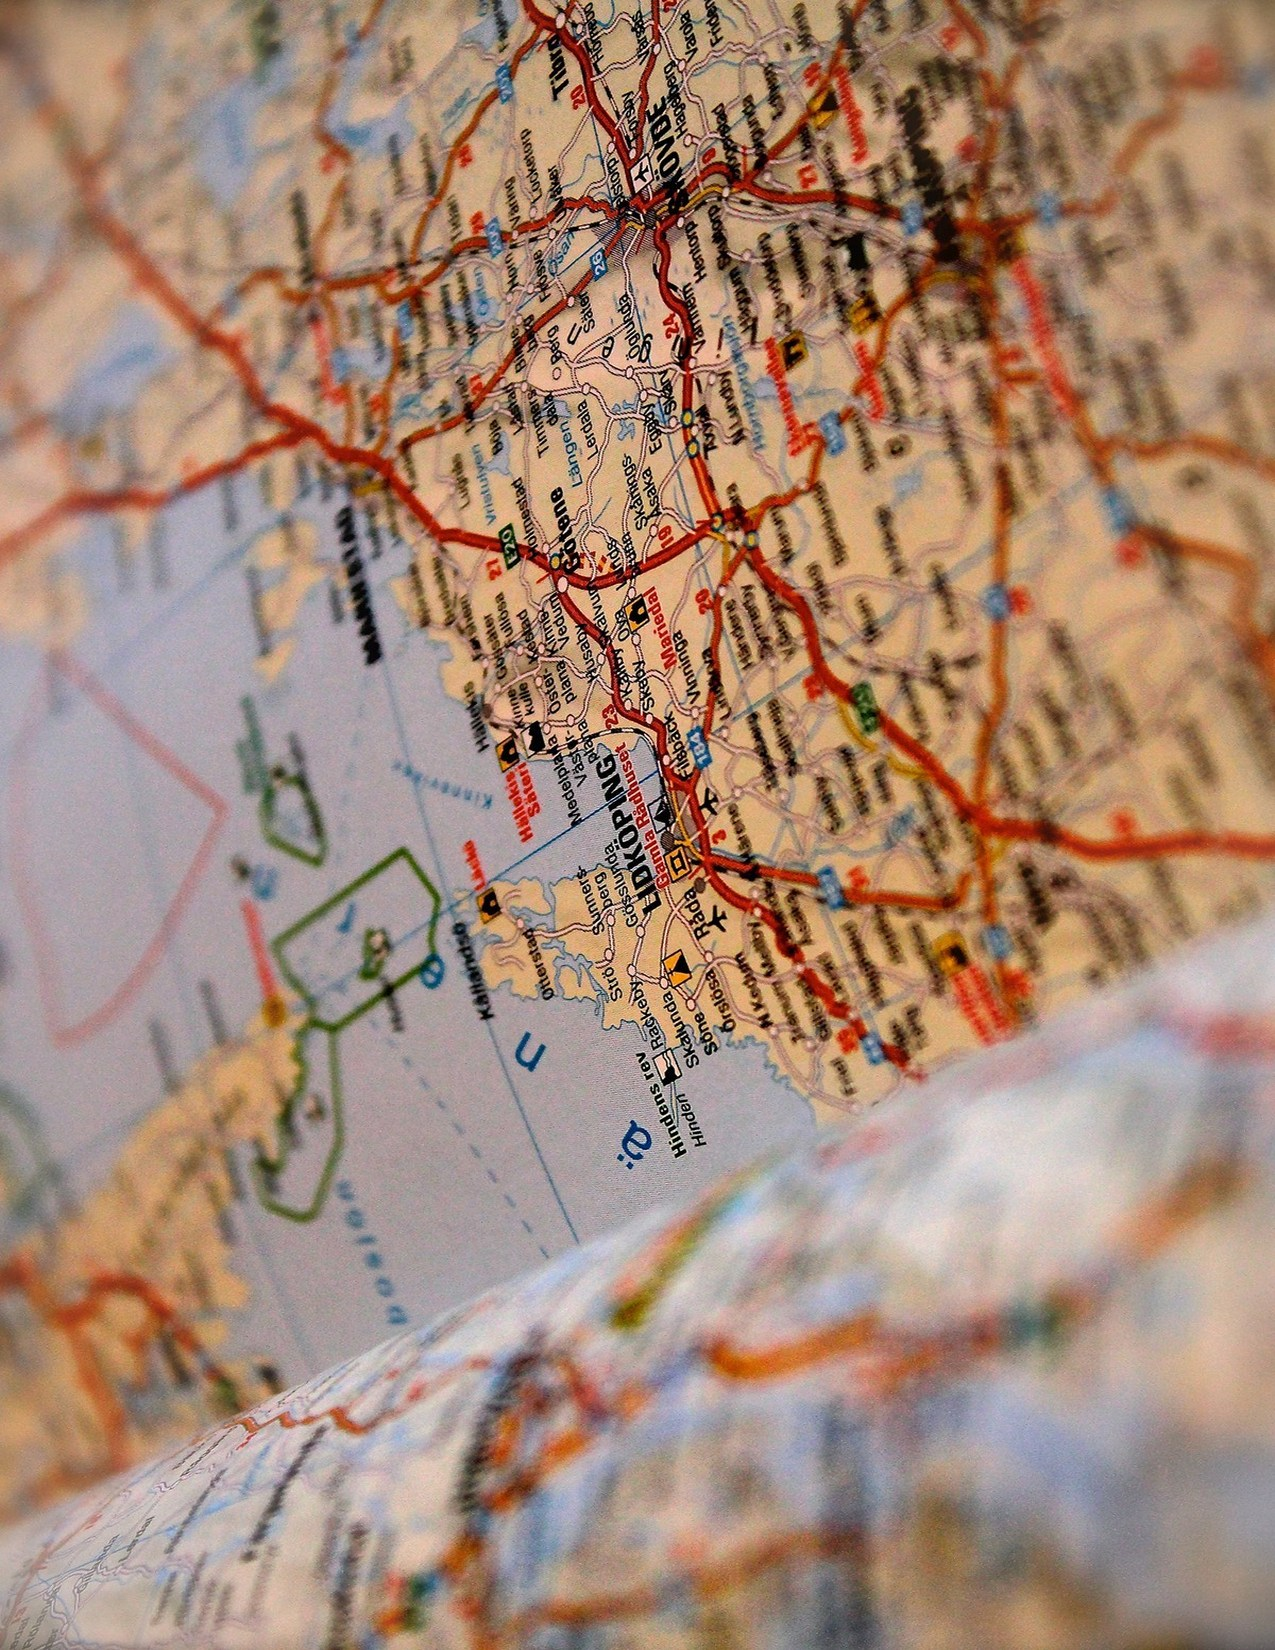
\includegraphics[scale=1.25]{903.jpg}}} % Image background
\centering
\vspace*{5cm}
\par\normalfont\fontsize{35}{35}\sffamily\selectfont
\textbf{Vehicle Routing Problems}\\
{\LARGE Analysis of Mathematical Models for VRP \& Derivatives}\par % Book title
\vspace*{1cm}
{\Huge Meet Pragnesh Shah}\par % Author name
\endgroup

%----------------------------------------------------------------------------------------
%	COPYRIGHT PAGE
%----------------------------------------------------------------------------------------

\newpage

\begin{figure}[h]
    \centering
    
\includegraphics[width=0.40\textwidth]{iima_logo.png}
    \end{figure}
    
~\vfill
\thispagestyle{empty}

%\noindent Copyright \copyright\ 2014 Andrea Hidalgo\\ % Copyright notice


\noindent \textsc{Winter Research Internship}\\

\noindent \textsc{Indian Institute of Management - Ahmedabad}\\

\noindent \textit{github.com/meetshah1995/IIMA-Intern}\\

\noindent This research was done under the supervision of Prof. Sachin Jayaswal within a total of 5 weeks, from November 26th of 2014 to January 1st of 2015\\ % License information

% Printing/edition date

%----------------------------------------------------------------------------------------
%	TABLE OF CONTENTS
%----------------------------------------------------------------------------------------

\chapterimage{904.jpg} % Table of contents heading image

\pagestyle{empty} % No headers

\tableofcontents % Print the table of contents itself

%\cleardoublepage % Forces the first chapter to start on an odd page so it's on the right

\pagestyle{fancy} % Print headers again

%----------------------------------------------------------------------------------------
%	CHAPTER 1
%----------------------------------------------------------------------------------------

\chapterimage{904.jpg} % Chapter heading image

\chapter{Introduction}

\section{Introduction}\index{Introduction}
The entire research internship duration was quite a walkthrough a lot of detailed MatheMatical Modelling of complex yet real-life optimization problems. Running an industry can be done even by a layman , but what takes you a mile ahead is how you use available resources judiciously and optimally and come up with ingenious methods of getting work done. One of many effects this research internship had on my mindset is that I got myself introduced to the genre of Operations Research both in theory and practical aspects.
\begin{quote}
This internship will have a long and lasting effect on the decisions I take in the future. I am completely thankful to Prof. Sachin Jayaswal to consider me worthy of the position and introduce me to this completely new genre in research : IEOR.
\end{quote}

\section{Abstract}\index{Abstract}
During my short stay at IIM , I touched the topic of Vehicle Routing and Travelling Salesman problems, then went into the intricacies of the mathematical models to describe these problems , their interpretations and analysis of different models and related complexities.
\vspace{.35cm}
\\This effort at research was a problem-based learning where I was supplied with several problems of varied genres under VRP to solve and hence get the chance to go through some very good papers on those topics varying from k-periodic symetric travelling salesman problems to vehicle routing problem with time windows.The allocation of problems in increasing order of Difficulty was extremely critical to the learning process alongside some good problem removal sessions with Sir. 
\vspace{.35cm}
\\I perused as much as 13 papers during my stay here and got an insight into the intricacies of Vehivle Routing Problem. I have given a brief literature review of each paper in the fore-coming sections which describes what made the paper unique and how it contributed to my learning process.

\newpage

\section{Software \& Packages Used}\index{Software \& Packages Used}

\begin{itemize}
\item Microsoft Excel
\begin{itemize}
\item OpenSolver
\item C-Solver
\end{itemize}
\item IBM CPLEX
\item AMPL
\end{itemize}

Each of these above tools for implementing and solving mathematical models is perfect in their own fields and I learnt that the choice of the tool to be used highly depends upon the problem statement and the format of the question.

\section{References}\index{References}

Since I was entirely new to this genre of research , I had to go through a couple of textbooks and popular papers on Vehicle Routing Problem and its derivatives. I have listed down a few popular papers below which I will be reviewing in this report.
\\*
\begin{itemize}

\item The two-period TSP applied to Milk-Collection in Ireland
\item Integer Programming formulations of multiple salesman problems
\item The Vehicle Routing Problem: An overview
of exact algorithms
\item A Survey on the Vehicle Routing Problem and
Its Variants
\item A Modelling and Optimization Framework for Real-World
Vehicle Routing Problems
\end{itemize}

\section{TextBooks}\index{Textbooks}

\begin{remark}
\textbf{Introduction to Operations Research}, \textit{Hiltier| Lieberman | Nag | Basu}, Third Edition, 2010.
\end{remark}
\begin{remark}
\textbf{Model Building in Mathematical Programming}, \textit{Williams}, Fifth Edition, 2010.
\end{remark}

%This statement requires citation \cite{book_key}; this one is more specific \cite[122]{article_key}.


%----------------------------------------------------------------------------------------
%	CHAPTER 2
%----------------------------------------------------------------------------------------
\chapterimage{904.jpg}

\chapter{Vehicle Routing Problem}

\section{First ideas}\index{First ideas}

  The vehicle routing problem (VRP) is a combinatorial optimization and integer programming problem seeking to service a number of customers with a fleet of vehicles. Proposed by Dantzig and Ramser in 1959, VRP is an important problem in the fields of transportation, distribution and logistics. Often the context is that of delivering goods located at a central depot to customers who have placed orders for such goods. The objective of the VRP is to minimize the total route cost.


Determining the optimal solution is an NP-complete problem in combinatorial optimization, so in practice heuristic and deterministic methods have been developed that find acceptably good solutions for the VRP. A non-technical explanation exists for why the VRP is much more challenging than might be expected.

\begin{figure}[h]
    \centering
    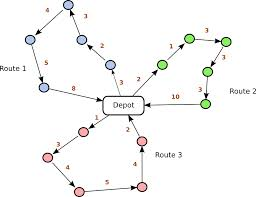
\includegraphics[width=0.77\textwidth]{download.jpg}
    \caption{Picuture of Single Depot n-Vehicle Routing , n=3. }
    \label{fig:awesome_image}
\end{figure}


\section{Derivatives of Vehicle Routing Problem}
Several variations and specializations of the vehicle routing problem exist:
\begin{itemize}
\item Travelling Salesman Problem (TSP):\\*
A TSP is essentially a VRP with a single depot and a single vehicle, in other words the TSP can be seen as an over-simplified version of the VRP and is perfect to start as a beginner to VRPs.

\item Vehicle Routing Problem with Pickup and Delivery (VRPPD):\\*
A number of goods need to be moved from certain pickup locations to other delivery locations. The goal is to find optimal routes for a fleet of vehicles to visit the pickup and drop-off locations.

\item Vehicle Routing Problem with LIFO: \\* 
Similar to the VRPPD, except an additional restriction is placed on the loading of the vehicles: at any delivery location, the item being delivered must be the item most recently picked up. This scheme reduces the loading and unloading times at delivery locations because there is no need to temporarily unload items other than the ones that should be dropped off.

\item Vehicle Routing Problem with Time Windows (VRPTW):\\* 
The delivery locations have time windows within which the deliveries (or visits) must be made. In computational complexity theory, this problem is known to be NP-hard.

\item Capacitated Vehicle Routing Problem (with or without Time Windows): CVRP or CVRPTW.\\*
The vehicles have limited carrying capacity of the goods that must be delivered.
Vehicle Routing Problem with Multiple Trips (VRPMT): The vehicles can do more than one route.

\item Open Vehicle Routing Problem (OVRP):\\*
Vehicles are not required to return to the depot.
Several software vendors have built software products to solve the various VRP problems. Numerous articles are available for more detail on their research and results.

\end{itemize}

\section{Indutrial Application of VRP and its derivatives}
The Application of the the VRP and its derivatives is boundless in today's era of door to door delivery. The very presence of better trasnport connectivity have boosted long distance business and hence burdened the transport section. With nations fighting over fossil fuel, it is of utmost priority to the transport section to use the fuels judiciously and engage lowest cost alongside maintaining customer satisfaction. A few day-to-day experiences where Vehicle Routing can save millions of rupees are :

\begin{itemize}

\item Bread Distibution
\item Online Market Supply Chain
\item Industrial Transport
\item Grains and vegetables Transport

\end{itemize}

\newpage

\section{Mathematical Model of Simple Vehicle Routing Problem}

\subsection{Model Definition}
In this section, the notation and formulation of the VRP are introduced. Let \(C = [1, 2, . . . , n]\) be the set of customers, each customer \(i\) with a positive integer demand
d{i}, and let \(V = [0] \cup C\), where 0 is the depot (with no demand). Each
\(arc (i, j) \hspace{.3cm} \forall  i, j \hspace{.3cm} \in  V\) has a nonnegative travel cost $c_{ij}$ (usually distances). These costs are assumed to satisfy the triangle inequality. The VRP is defined on a directed graph \(G = (V, A)\), where A is the set of \(arcs [(i, j) \hspace{.3cm}/ i, j \in V,\hspace{.3cm} i hspace{.3cm}j = 6]\). A set of \(K\) identical vehicles, each with capacity \(Q \in Z^{+}\),  is available at the depot.We assume that K is equal to \(K_{min}\), the minimum number of vehicles needed to
serve all the customers, which is determined as \(K_{min} = \frac{d(C)}{Q_{e}}\), where d(C) is
the sum of all the demands.\\
\vspace*{.5cm}
The objective function is the total travel cost and can be expressed as :\\
\hspace*{5cm} \(\sum\limits_{(i,j) \in A} \sum\limits_{k=1}^{K} c_{ij}x_{ijk}\)\\

where $x_{ij}$ is a binary variable that takes value one if vehicle $k$ travels directly from $i$ to $j$ (and zero otherwise). Defining variables $y_{ik} \geq 0$ as the demand of customer $i \in C$ delivered by vehicle $k = 1, 2, . . . , K,$ the vehicle flow formulation for the VRP :\\


\begin{align}
\min & \sum_{(i,j) \in A} \sum\limits_{k=1}^{K} c_{ij}x_{ijk}\\
s.t.& \sum\limits_{i \in I} \sum\limits_{k=1}^{K} x_{ijk} \geq 1 && & \forall j \in C\\
& \sum\limits_{j \in I} \sum\limits_{k=1}^{K} x_{0jk} = K && \\
& \sum\limits_{i \in I}x_{ipk} - \sum\limits_{j \in I} x_{pjk} = 0 && & p \in I, k = 1,2,3,4....K\\
& \sum\limits_{i \in S} \sum\limits_{j \in S}x_{ijk} \leq |S|-1 && & S \subseteq C, k = 1,2,3,4....K\\
& y_{ik} \leq d_{i}\sum\limits_{j \in I}x_{ijk} && & \text{$i \in C, k = 1,2,3,4....K $}\\
& \sum\limits_{i \in C}y_{ik} \leq Q && & \text{$ k = 1,2,3,4....K $}\\
& \sum\limits_{k = 1}^{K}y_{ik} = d_{i} && & \text{$i \in C $}\\
& x_{ijk} \in \{0,1\}  && & \text{$(i, j) \in A, k = 1,2,3,4....K $}\\
& y_{ik} \geq 0  && & \text{$i \in C, k = 1,2,3,4....K $}
\end{align}

\newpage

\subsection{Constraints and their Interpretation} 
\begin{itemize}
\item (2.1) state that every customer must be visited by at least one
vehicle 
\item (2.2) impose that exactly K routes are performed.
\item(2.3) indicate that if vehicle k visits node p, then it must leave it (flow conservation constraints) 
\item(2.4) are the classical subtour elimination constraints.
\item(2.5) guarantee that the customer can only be served if the vehicle visits it.
\item(2.6) limit to Q the maximum load of each vehicle while
\item(2.7) ensure that the entire demand of each node is satisfied.
\end{itemize}


\subsection{Implementation in IBM CPLEX}

\begin{lstlisting}
/*********************************************************************
 *Vehicle Routing Problem
 *6 employees, 1 Office, minimum 2 tours for 3-seater cars.
 *Author : meetshah1995
 * Min Sum[i,j](Cij*Xijk) s.t.
 *		Sum[i,i!=j](Xijk)=1
 *		Sum[j,i!=j](Xijk)=1
 *		Sum[k,i!=j](Xijk)=1
 *		Sum[i]Sum[k](Xi7k)=2
 * 		Sum[j]Sum[k](X7jk)=2
 *		0<=Xij<=1
 ********************************************************************/
#include<stdio.h>
#include<conio.h>
#include<iostream>
#include<fstream>
#include<iosfwd>
#include<string>
#include <deque>
#include <sstream>
#include <time.h>
#include <stdlib.h>
#include <vector>//for vectors
#include <math.h>
#include <cplex.h>
#include <ilcplex/ilocplex.h>
#include <ilconcert/ilosys.h>

using namespace std;

ILOSTLBEGIN

int main(int argc, char **argv) 
{
	IloEnv env;
    try 
	{
		IloArray<IloNumArray> distance(env);
		
		//Model Initialization
		IloModel model(env);


		//Taking Data from Distance Data File
		ifstream in;
		in.open("carpool-data.txt",ios::in);
		in >> distance;
		in.close();
		cout<<distance<<endl;
		
		//2D Array for Results
		IloArray<IloNumArray> X_val(env, 7);
		for (int i = 0; i < 7; i++)
		{
			X_val[i] = IloNumArray(env,7);
		}

		IloArray<IloNumArray> Y_val(env, 7);
		for (int i = 0; i < 7; i++)
		{
			Y_val[i] = IloNumArray(env,7);
		}

		//2D Array for Xij
		IloArray<IloNumVarArray> X(env, 7);
		for (int i = 0; i < 7; i++)
		{
			X[i] = IloNumVarArray(env,7,0,1,ILOINT);
		}

		//2D Array for Yij
		IloArray<IloNumVarArray> Y(env, 7);
		for (int i = 0; i < 7; i++)
		{
			Y[i] = IloNumVarArray(env,7,0,1,ILOINT);
		}


		// Defining Obj to be equal to sum-product(Dij*Xij)
 		IloExpr Obj(env);
 		for (int i = 0; i < 7; ++i)
 		{
 			for (int j = 0; j < 7; j++)
 			{
 				Obj += distance[i][j]*X[i][j];
 			}
 		}
		
		for (int i = 0; i < 7; ++i)
 		{
 			for (int j = 0; j < 7; j++)
 			{
 				Obj += distance[i][j]*Y[i][j];
 			}
 		}

		IloObjective Objective = IloMinimize(env); 
		model.add(Objective); 
		Objective.setExpr(Obj);
		Obj.end();

		//Constraints for the model

		//Ensuring that one edge is only on one tour
		IloExpr Exclusion(env);
		for (int i = 0; i < 7; i++)
		{
			for (int j = 0; j < 7; j++)
			{
				Exclusion += X[i][j] + Y[i][j];
				model.add(Exclusion == 1);
			}
		}
		Exclusion.close();

		//outgoing
		for (int i = 0; i < 7; i++)
		{
			IloExpr Sum(env);
			for (int j = 0; j < 7; j++)
			{
				if(i != j)
					Sum += X[i][j];
			}
			model.add(Sum == 1);
			Sum.end();	
		}

		for (int i = 0; i < 7; i++)
		{
			IloExpr Sum(env);
			for (int j = 0; j < 7; j++)
			{
				if(i != j)
					Sum += Y[i][j];
			}
			model.add(Sum == 1);
			Sum.end();	
		}

		//incoming
		for (int j = 0; j < 7; j++)
		{
			model.add(X[j][j]==0);
			IloExpr Sum(env);
			for (int i = 0; i < 7; i++)
			{
				if(i != j)
					Sum += X[i][j];
			}
			model.add(Sum == 1);
			Sum.end();	
		}



		for (int j = 0; j < 7; j++)
		{
			model.add(Y[j][j]==0);
			IloExpr Sum(env);
			for (int i = 0; i < 7; i++)
			{
				if(i != j)
					Sum += Y[i][j];
			}
			model.add(Sum == 1);
			Sum.end();	
		}

		//Ensuring 2 entries and exits for the Office node
		IloExpr Double(env);
		for (int i = 0; i < 7; i++)
		{
			Double += X[6][i];
			Double += X[i][6];
		}
		for (int i = 0; i < 7; i++)
		{
			Double += Y[6][i];
			Double += Y[i][6];
		}
		model.add(Double == 2);
		Double.end();

		//SECs
		/*for (int i = 1; i < 7; i++)
		{
			for (int j = 1; j < 7; j++)
				if(i!=j)
			{
				IloExpr sec(env);
				sec = U[i] - U[j] +7*X[i][j];
				model.add(sec <= 6);
				sec.end();
			}
		}*/

		// Optimize
		IloCplex cplex(model);
		cplex.setOut(env.getNullStream()); // if we get an empty stream in return
		cplex.solve();//solving the MODEL
		if (cplex.getStatus() == IloAlgorithm::Infeasible) // if the problem is infeasible
		{
			env.out() << "Problem Infeasible" << endl; 
		}
		for(int i = 0; i < 7 ; i++)
		{
			cplex.getValues(X_val[i], X[i]);
		}
		cout<<X_val<<endl;
		// Print results
		cout<< "Objective Value = " << cplex.getObjValue() << endl;
		cout<<"X = "<<X_val<<endl;
	}
	catch(IloException &e) 
	{
		env.out() << "ERROR: " << e << endl;
	}
	catch(...)
	{
		env.out() << "Unknown exception" << endl;
	}
	env.end();
	return 0;
}
\end{lstlisting}

%----------------------------------------------------------------------------------------
%	CHAPTER 4
%----------------------------------------------------------------------------------------

\chapterimage{904.jpg} % Chapter heading image

\chapter{Paper Reviews}

\section{The two-period TSP applied to Milk-Collection in Ireland}
Author(s) : Martin Butler, Paul Williams \& Leslie-Ann Yarrow \\
        
        In this classical paper , the author gives a mild introduction to k-period symmetric TSPs and then builds on them to apply the same model on Milk Collection in Ireland.\\

The paper essentially is a problem solving technique for 2 period symmetric TSP which needs an optimal route for milk collection where there are a few \textit{everyday farms} which have to be visited daily and a few \textit{everyday other farms} which have to be visited only once in two days. Using a clever implementation of the famous MTZ subtour elimination constraints , this problem is essentially shortened to a Multiple Traveling Salesman Problem.  

\section{Integer Programming formulations of multiple salesman problems}
Author(s) : Imdat Kara \& Tolga Bektas \\
        
        In this paper, the authors extend the classical multiple traveling salesman problem (mTSP) by imposing a minimal number of nodes that a traveler must visit as a side condition. Single and multidepot cases and propose integer linear programming formulations for both, with new bounding and subtour elimination constraints. It is shown that several variations of the multiple salesman problem can be modeled in a similar manner. Computational analysis shows that the solution of the multidepot mTSP with the proposed formulation is significantly superior to previous approaches.\\

This paper is a example of power of \textit{Kulkarni \& Bhave } subtour eliminiation constraints. This example shows the excellence of \textit{Kulkarni \& Bhave } SECs over MTZ SECs in standard TSPs both in number constraints and space complexity.

\section{The Vehicle Routing Problem: An overview
of exact algorithms }
Author(s) : Gilbert Laporte \\
        
        In this classical must-read TSP paper , the author gives an extremely detailed introduction to solution methods to symmetric TSPs, which generally form the  .\\

The paper essentially is a problem solving technique for 2 period symmetric TSP which needs an optimal route for milk collection where there are a few \textit{everyday farms} which have to be visited daily and a few \textit{everyday other farms} which have to be visited only once in two days. Using a clever implementation of the famous MTZ subtour elimination constraints , this problem is essentially shortened to a Multiple Travelling Salesman Problem.


\section{A Survey on the Vehicle Routing Problem and
Its Variants}

Author(s) : Suresh Nanda Kumar \& Ramasamy Panneerselvam\\
        
        This paper exhaustively enlists all the possible variants of the VRP, which find application in the industrial logistics optimization.\\
        
        This paper conducts a literature review on the recent developments and publications involving the vehicle
routing problem and its variants, namely vehicle routing problem with time windows (VRPTW) and the capacitated vehicle routing problem (CVRP) and also their variants. The VRP is classified as an NP-hard problem. Hence, the use
of exact optimization methods may be difficult to solve these problems in acceptable CPU times, when the problem involves real-world data sets that are very large. The vehicle routing problem comes under combinatorial problem.
Hence, to get solutions in determining routes which are realistic and very close to the optimal solution, examples of using heuristics
and meta-heuristics are given. In this paper we discuss the various exact methods and the k-opt heuristics and meta-heuristics used to solve the VRP and its variants.
        
\section{A new approach to solving the multiple traveling salesperson problem using genetic algorithms}

Author(s) : Arthur E. Carter \& Cliff T. Ragsdale \\
        
        In this revolutionary and intellectual stimulating paper , the authors gives a mild introduction to well known Genetic Algorithms and cleverly applies a them to solve the multiple travelling salesman problem with it using lower computational power and producing similar results.\\
. 

This paper focuses on solving the MTSP with genetic algorithms (GAs) using standard TSP chromosomes and operators. This paper proposes a new GA chromosome and related operators for the MTSP and compares the theoretical properties and computational performance of the proposed technique to previous work. Computational testing shows the new approach results in a smaller search space and, in many cases, produces better solutions than previous techniques. This technique can serve as a basic solver for huge databases as the space complexity of the algorithm is almost neglible as to standard Mathematical Model solving using MTZ constraints as described in 3.2 .

\vfill
\hspace*{5cm} \textit{Cheers, Meet Shah}
\end{document}